\documentclass[letterpaper,12pt]{article} %tipo de documento y tama~o de papel y letra
\usepackage[latin1]{inputenc} %codificacion de caracteres
\usepackage[spanish]{babel} %idioma
\usepackage{fancyhdr} %tipo de pagina, LINDA biggrin.gif
\usepackage[top=3.5cm,bottom=2.5cm,right=2cm,left=2.5cm]{geometry} %margenes
\usepackage[rflt]{floatflt} %ni puta idea
\usepackage{pdfpages} %incluir archivos pdf
\usepackage{hyperref} %hipervinculos
\hypersetup{
  colorlinks=true,
  urlcolor=cyan
}
%\usepackage{helvet} %esto es pa escribir con Arial en vez de times new roman
%\renewcommand\familydefault{\sfdefault} %descomenta estas lineas para escribir en arial

\usepackage{multirow}

\usepackage{graphicx} %para usar imagenes
%\newcommand{\imgdir}{doc-img} % para meter las imagenes en una carpeta especial, tunz en la carpeta del documento tiene q ir otra que se llame 'doc-img'
\graphicspath{{./pic/}} %le dice que las imagenes estan en la carpeta de arriba

\usepackage{amsmath} %pa usar smbolos matematicos
\numberwithin{equation}{section} % pa usar ecuaciones de modo lindo
\numberwithin{figure}{section} %para agregar imagenes
\numberwithin{table}{section} %para agregar tablas

\usepackage{subfigure} % pa usar sub figuras



\pagestyle{fancy} %configuracion para la pagina linda
\renewcommand{\sectionmark}[1]{\markboth{}{\thesection\ \ #1}} %cambios de comentarios
\lhead{} %parte de arriba, izq
\chead{} %parte de arriba, centro
\rhead{\rightmark} %parte de arriba, derecha, le agrega la marca del capitulo
\lfoot{} %parte de abajo, izq
\cfoot{} %parte de abajo, centro
\rfoot{\thepage} %parte de abajo, derecha, va el numero de la pagina


%-------------portada---------------------------------%
\begin{document}
\begin{titlepage} %portada
\thispagestyle{empty} %borrar el formato de pagina linda
%\begin{flushleft} %alinear a la izq
\begin{center}

\includegraphics[scale=0.35]{logoUSM-DI.eps}
%\vfill
\end{center}
%\end{flushleft}

\vspace{3cm} %espacio vertical , en realidad es un enter de 2 cm
\begin{center} %centrar
{\Huge Requerimientos de Software \\
 \huge Proyecto ``\emph{V.I.Pe.R.}''\\
  \normalsize\today
}
\end{center}

\vspace{6cm}

\vfill
\begin{flushleft} %alinear derecha
Pre-Empresa: \emph{Phyrex}\\
Jefe de Proyecto: Rodrigo Fr\'{\i}as\\
Integrantes:
\begin{table}[hb]
  \begin{tabular}{lcc}
    Rodrigo Fr\'{\i}as & \texttt{\small <rodrigo.frias@alumnos.usm.cl>} & [+56 9 83988257] \\
    Celeste Bertin & \texttt{\small <celeste.bertin@alumnos.usm.cl>} &[+56 9 68410901]\\
    Patricio Carrasco &\texttt{\small <patricio.carrascod@alumnos.usm.cl>} &[+56 9 50626689]\\
    Rocio Fernandez &\texttt{\small <rocio.fernandezu@alumnos.usm.cl>} & [+56 9 62426549]\\
    Juan Avalo & \texttt{\small <juan.avalo@alumnos.usm.cl>} & [+56 9 ]\\
  \end{tabular}
\end{table}
\end{flushleft}
\end{titlepage}
%------------------fin de la portada --------------------%

%{\bf } %escribir en negrita

\setcounter{page}{1} %empezar enumerando la pagina 1

\tableofcontents
\newpage

\section{Ficha de Clasificaci\'on R\'apida}
\subsection{Objetivo del Proyecto} %140 caracteres
\subsection{Resumen del Proyecto} %media pagina
\subsection{Cliente}
Nombre: Jocelyn Simmonds\\
Cargo: \\
E-mail: jsimmond@inf.utfsm.cl\\
Tel\'efono: \\
Rol o Experiencia relevante al producto:

\newpage
\section{Modelo de Dominio}

\begin{figure}
   \centering
     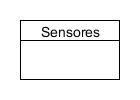
\includegraphics[scale=0.5]{ModeloDominio.jpg}
   \caption{}
   \label{fig:ModeloDominio}
\end{figure}


\begin{table}[hb!]
  \begin{tabular}{lp{7cm}}\hline
    Entidad & Descripci\'on \\ \hline \hline %1 linea
    & \\ \hline
  \end{tabular}
\end{table}

\newpage
\section{Actores y Tareas Clave}

\begin{table}[hb!]
  \begin{tabular}{lp{7cm}}\hline
    Actor & Descripci\'on \\ \hline \hline %1 linea
    & \\ \hline    
  \end{tabular}
\end{table}

\begin{table}[hb!]
  \begin{tabular}{lp{7cm}}\hline
    Tarea Clave & Descripci\'on \\ \hline\hline %max 3 lineas
    & \\ \hline
  \end{tabular}
\end{table}

\newpage
\section{Requerimientos Extra-funcionales}

\begin{table}[hb!]
  \begin{tabular}{lp{7cm}}\hline 
    Req. Extra-funcional & Descripci\'on y medici\'on \\ \hline\hline %max 2 lineas
    & \\ \hline
  \end{tabular}
\end{table}

\newpage
\section{Restricciones de Software y Hardware}

\begin{table}[hb!]
  \begin{tabular}{lp{7cm}}\hline
    Restricci\'on & Raz\'on \\ \hline\hline %max 2 lineas
    & \\ \hline
  \end{tabular}
\end{table}

\newpage
\section{Casos de Uso} %al menos 3 casos de uso no-triviales

\begin{figure}
   \centering
     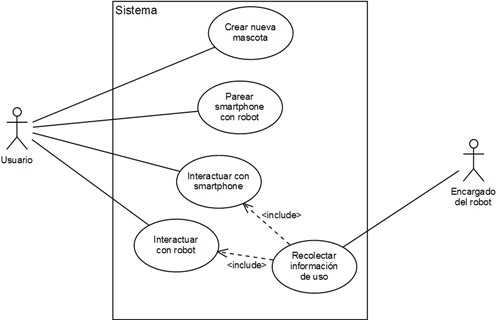
\includegraphics[scale=0.5]{CasoUso.jpg}
   \caption{}
   \label{fig:CasoUso}
\end{figure}


\begin{table}[hb!]
  \begin{tabular}{p{3cm}p{7cm}}\hline\hline
    Nombre: &  \\ \hline
    Descripci\'on: & \\ \hline %max 5 lineas
    Pre-condiciones: & \\ \hline
    Post-condiciones: & \\ \hline
    Requerimienos no Funcionales: & \\ \hline\hline %min 0 ; max 3
  \end{tabular}
\end{table}

\begin{table}[hb!]
  \begin{tabular}{p{3cm}p{7cm}}\hline\hline
    Nombre: &  \\ \hline
    Descripci\'on: & \\ \hline %max 5 lineas
    Pre-condiciones: & \\ \hline
    Post-condiciones: & \\ \hline
    Requerimienos no Funcionales: & \\ \hline\hline %min 0 ; max 3
  \end{tabular}
\end{table}

\begin{table}[hb!]
  \begin{tabular}{p{3cm}p{7cm}}\hline\hline
    Nombre: &  \\ \hline
    Descripci\'on: & \\ \hline %max 5 lineas
    Pre-condiciones: & \\ \hline
    Post-condiciones: & \\ \hline
    Requerimienos no Funcionales: & \\ \hline\hline %min 0 ; max 3
  \end{tabular}
\end{table}



%\newpage
%\chapter*{Anexo I - Presentaci\'on} %Copia Presentacion
%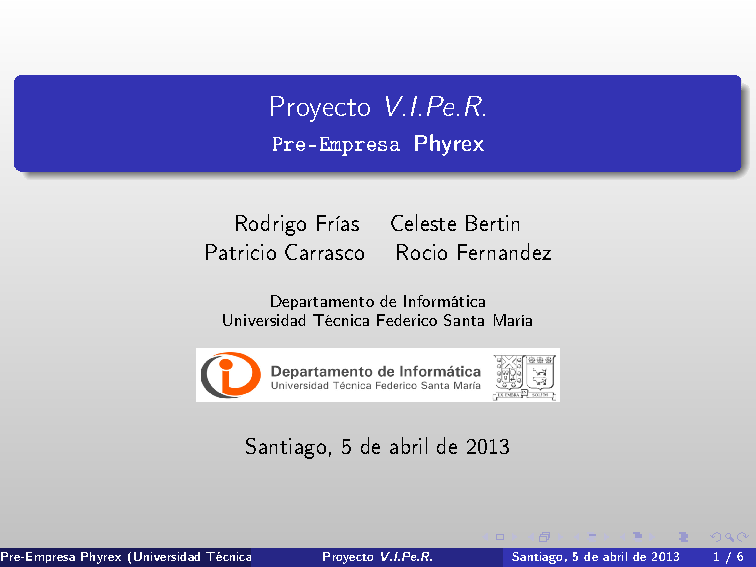
\includepdf[pages={1-},frame=true,nup=2x3,delta=10 20,scale=0.85]{../Presentacion/diapo-1x1.pdf}
%\newpage
%\chapter*{Anexo II - Curr\'{\i}culum Vitae} %Curriculum
%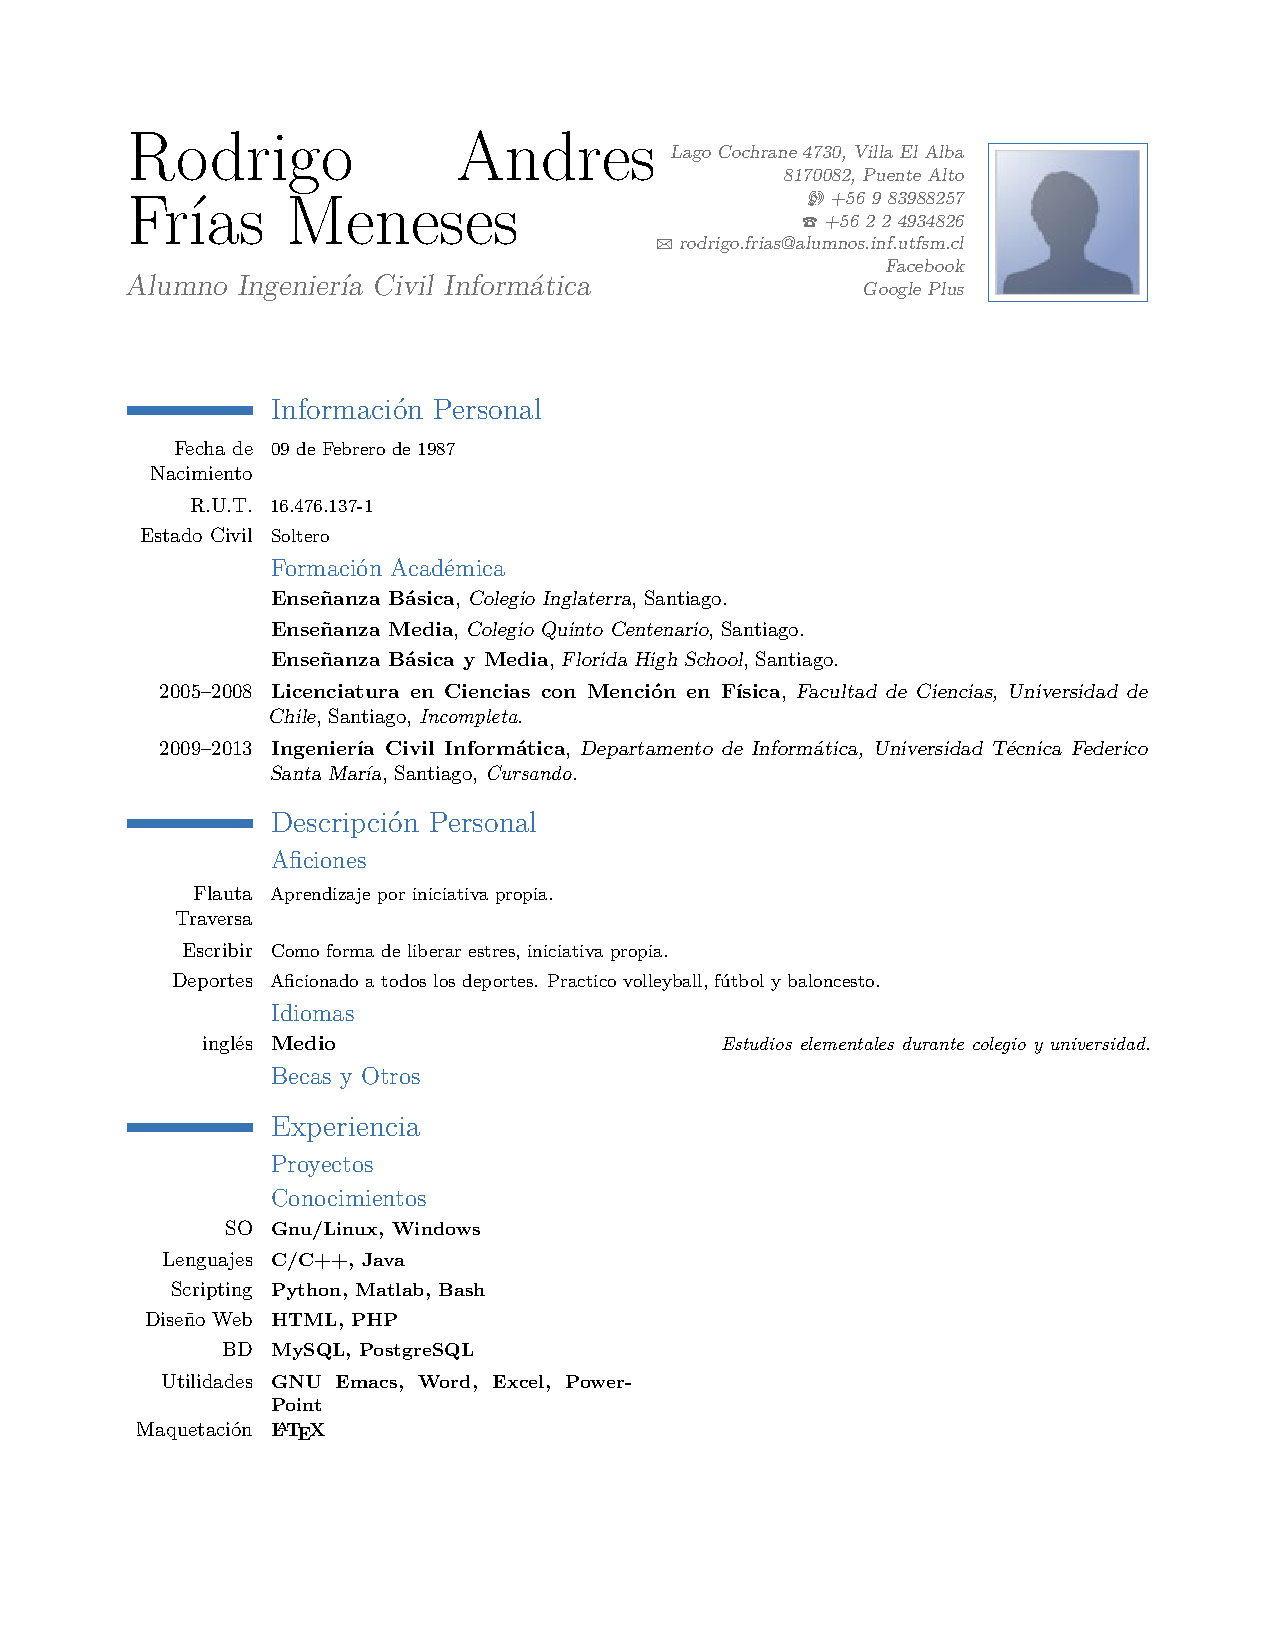
\includepdf[pages={1}]{../CV/cv-igo.pdf}
%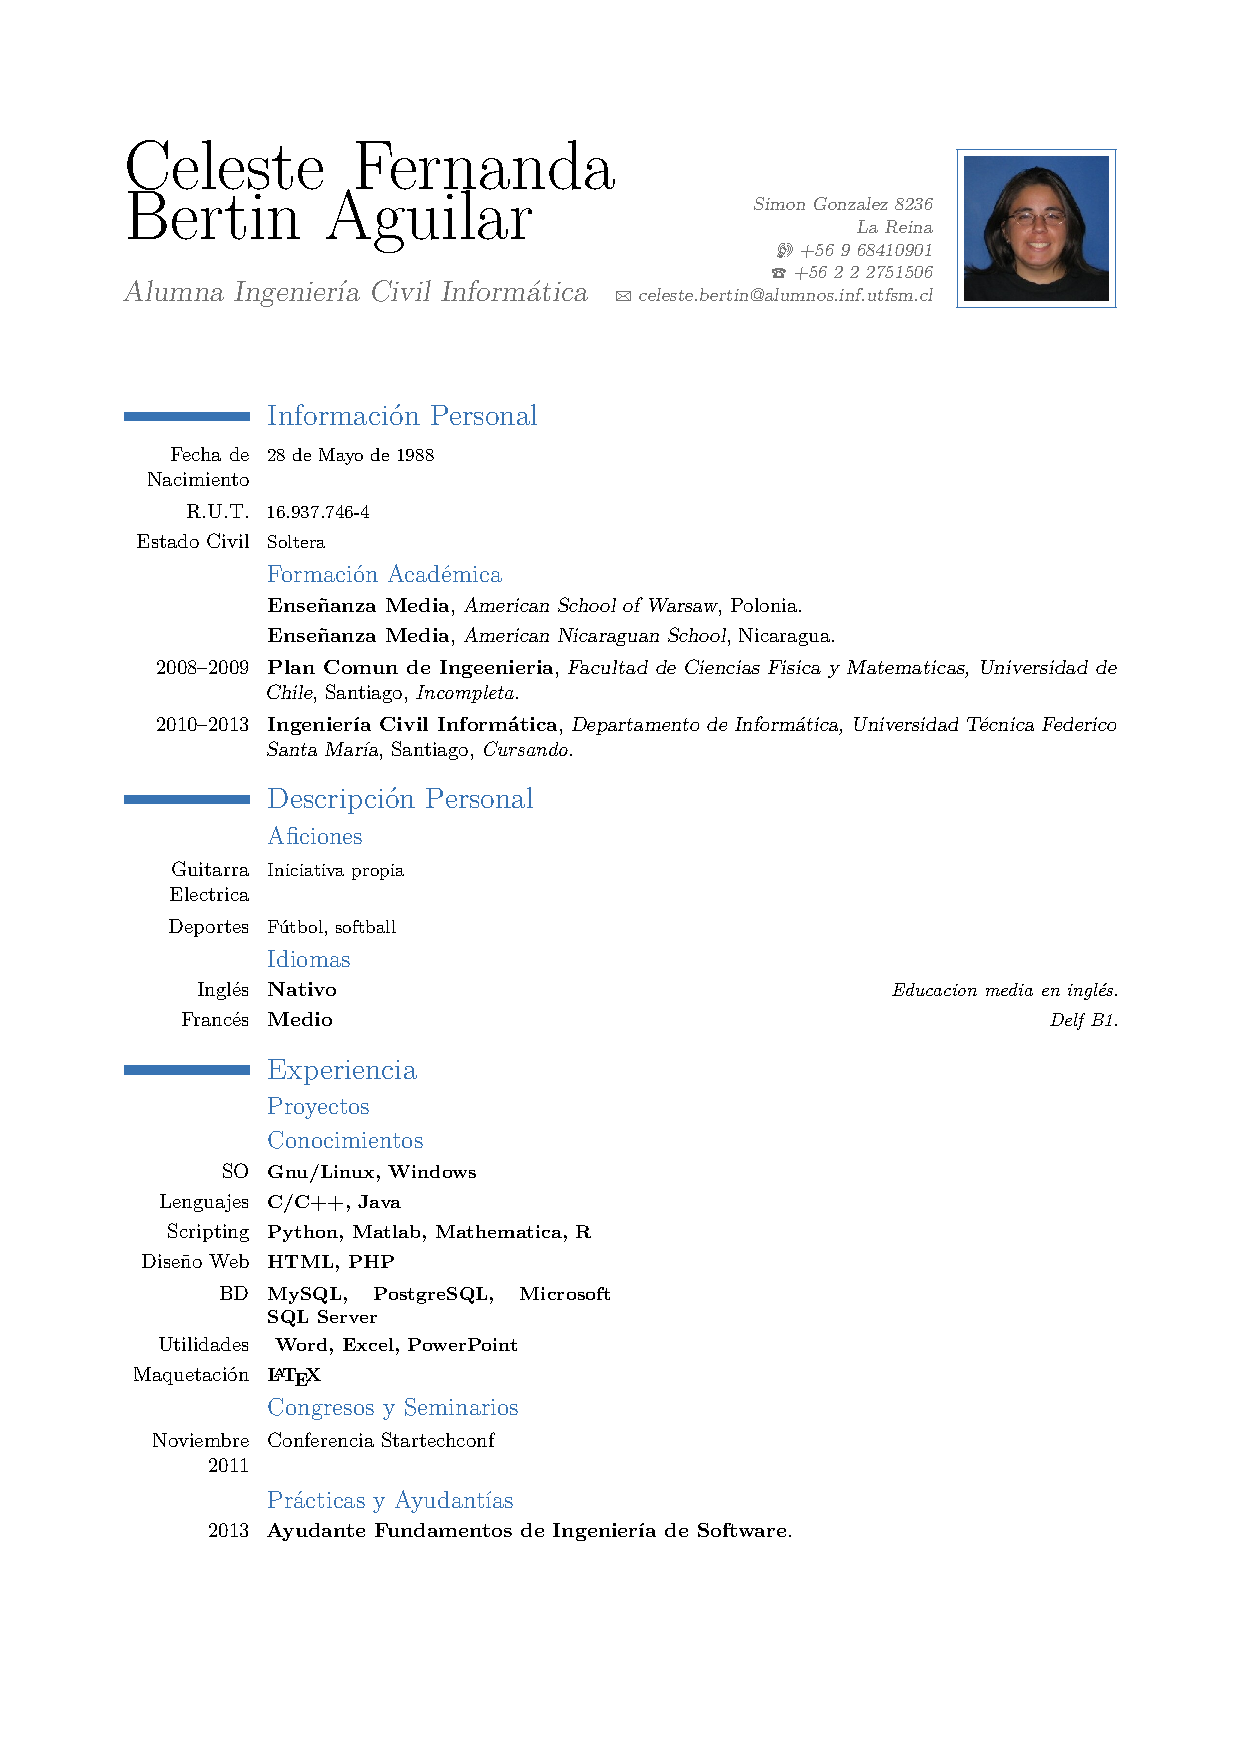
\includepdf[pages={1}]{../CV/cv-celeste.pdf}
%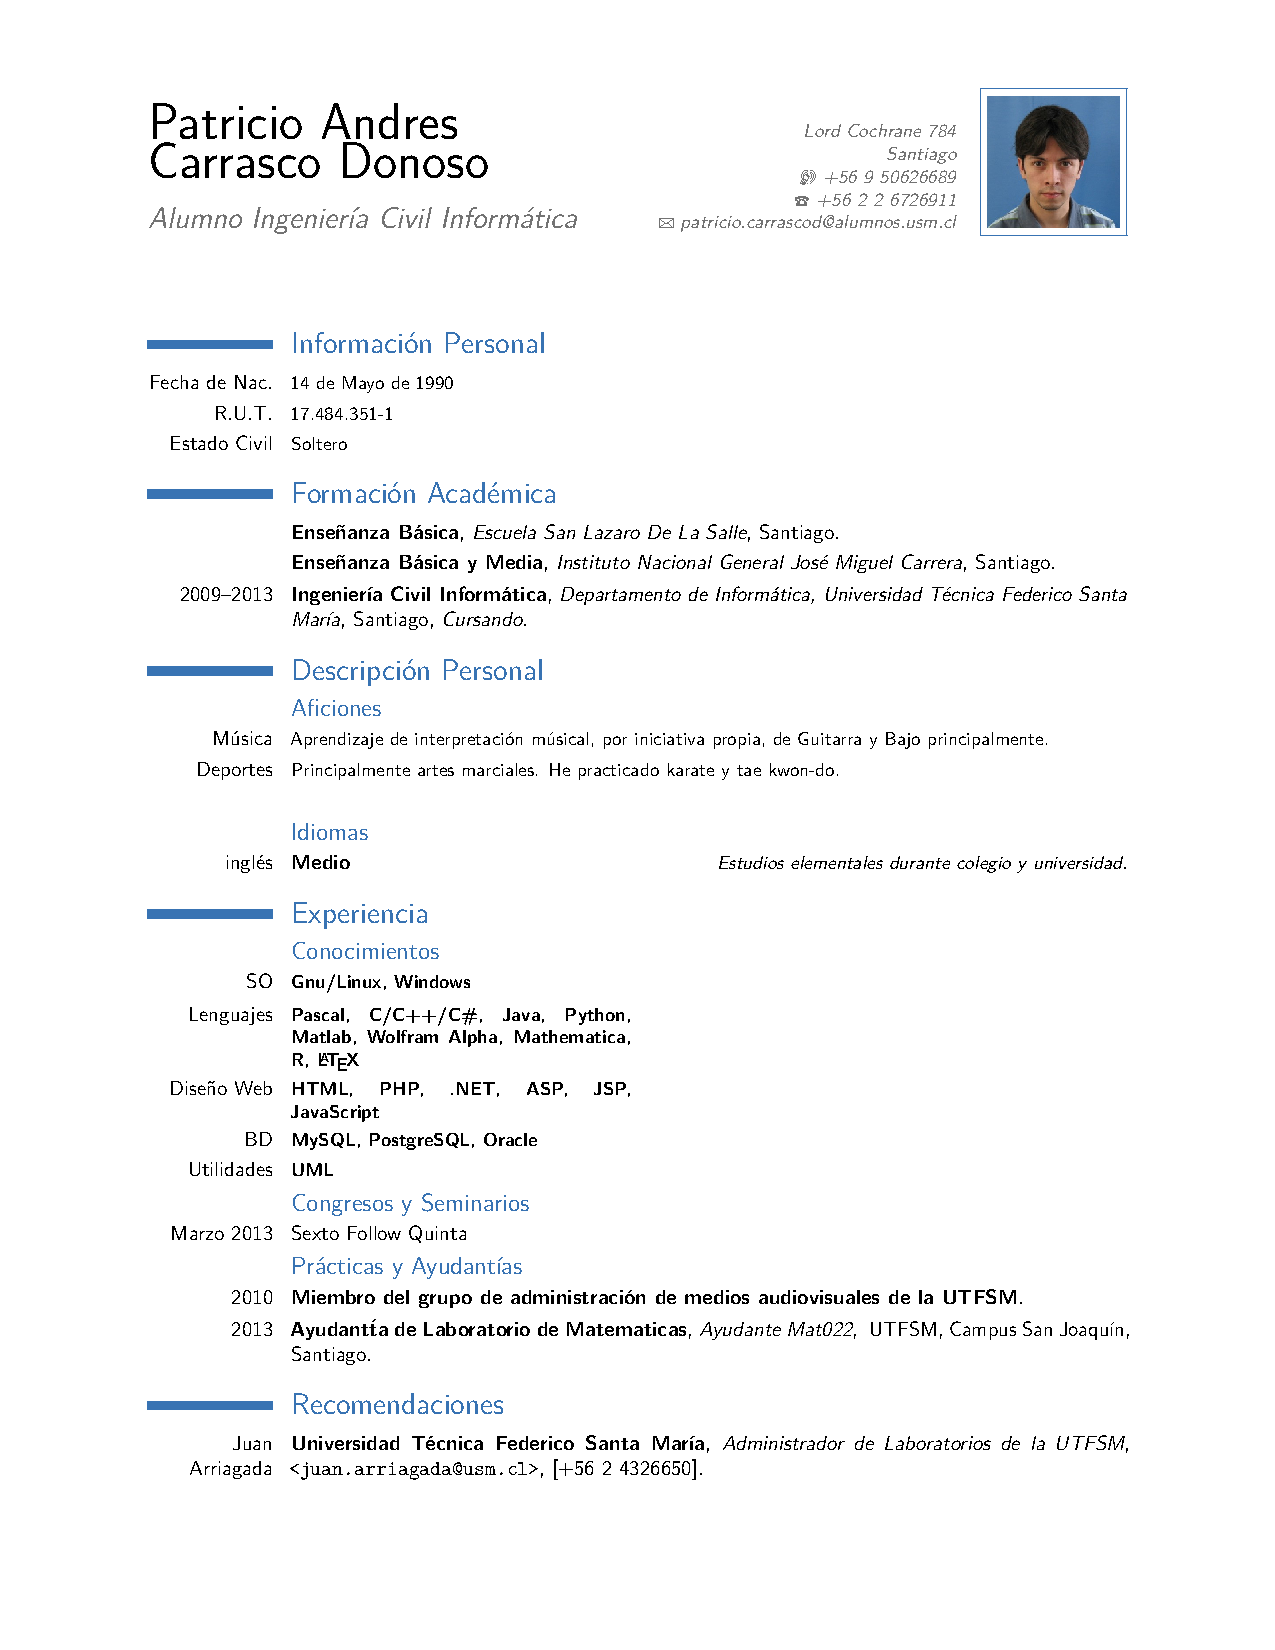
\includepdf[pages={1}]{../CV/cv-pato.pdf}
%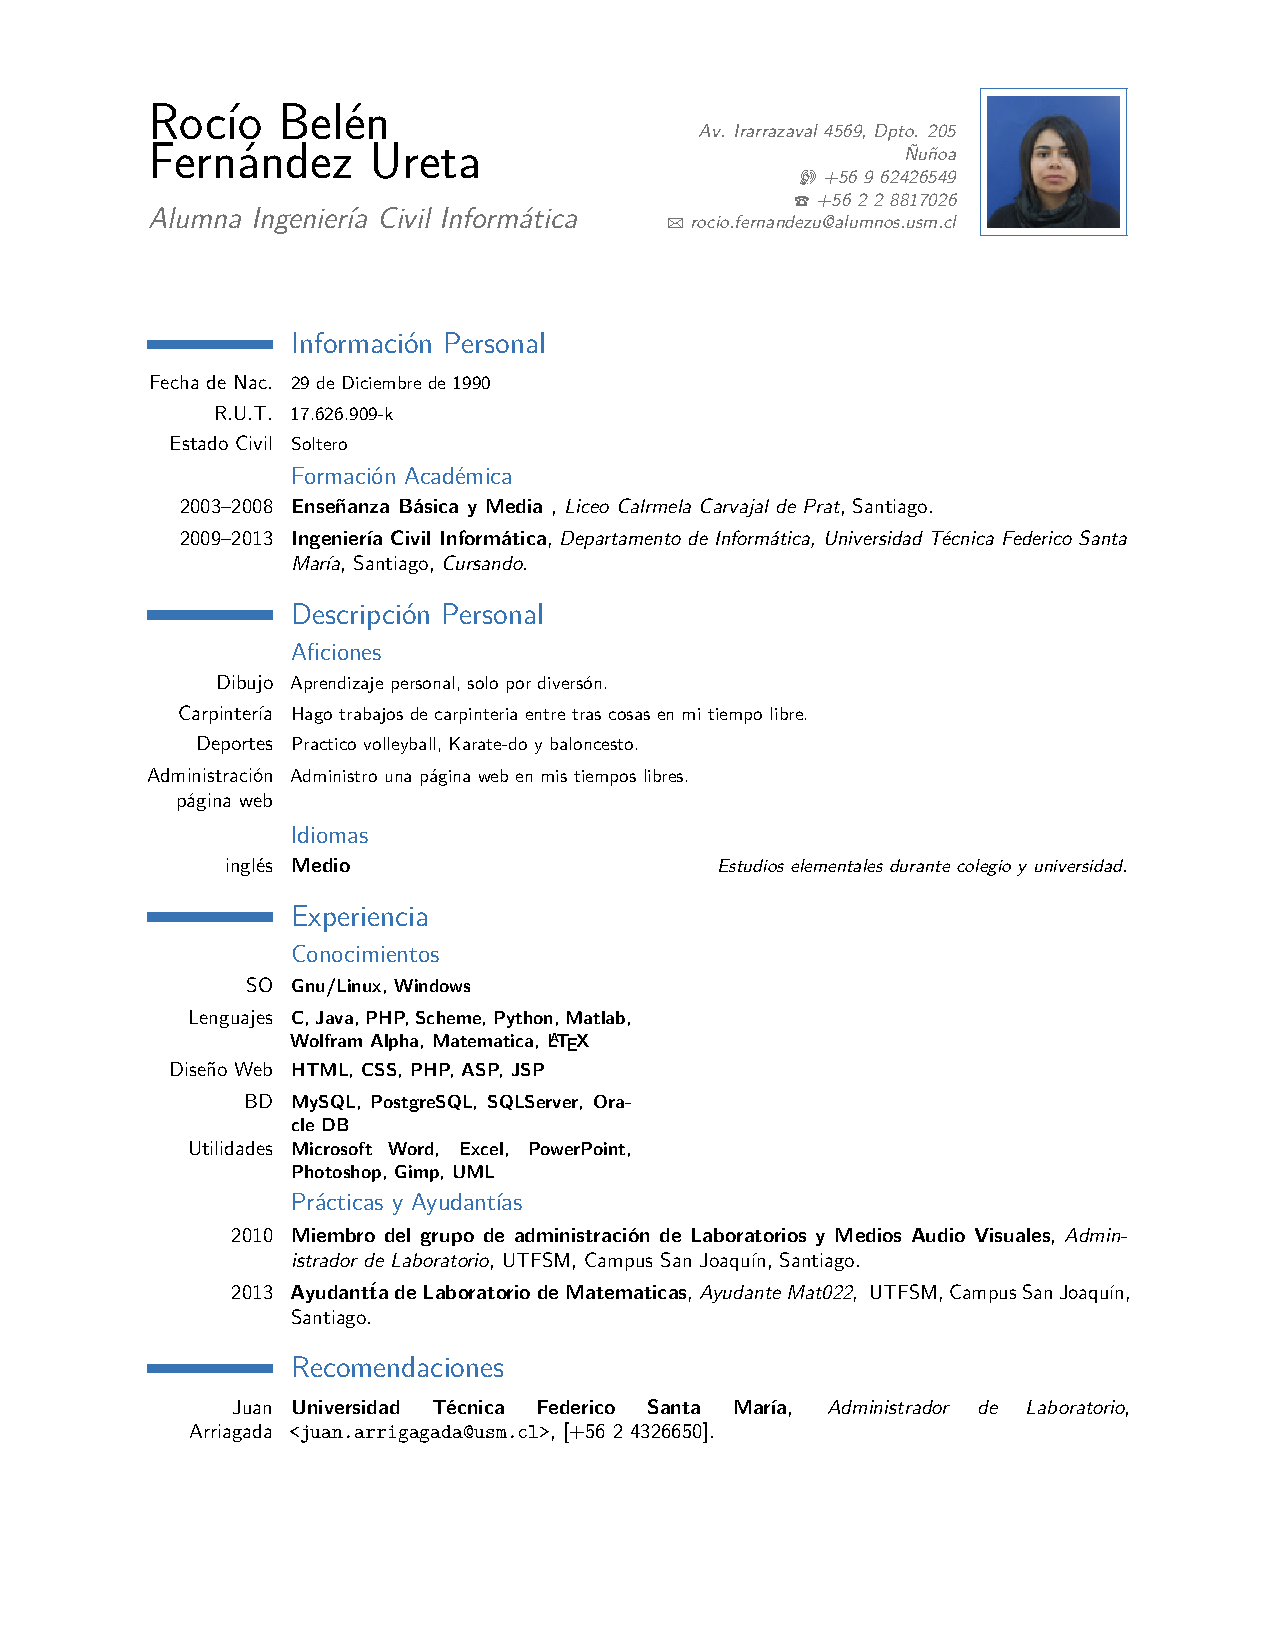
\includepdf[pages={1}]{../CV/cv-neko.pdf}
%\newpage
%\chapter*{Anexo III - Otros} %Otros


\end{document}
